\chapter{Mapping the Brain: A review of brain parcellations}
\label{ch:brain_mapping}

\section{Overview}
Neuroscientists have long thought of the brain as a mosaic of spatially contiguous
regions. How to define such regions is a hot topic in modern neuroscience.
Different brain parcellations exist based on criteria such as anatomy,
cytoarchitecture or functional specialization~\cite{Brodmann1909, Collins1998, Yeo2011}.
In this chapter, we introduce the main topic of our thesis: brain
parcellation. We review the main criteria used to divide the brain, the methodology
used to create brain parcellations under each criteria, and some widely used
brain parcellations.

\section{Introduction}
Composed of billions of interconnected neurons, the brain is a highly complex
biological machine. Untangling this network is the main goal of
neuroscience, a task that has proven to be arduous. The problem is two fold.
First, it is not feasible to characterize cellular function or axonal
connectivity at the scale of the brain with current approaches. Second, even if
we could characterize the neural network at a cellular level, studying it is
unrealistic given the huge amount of neurons in the brain~\cite{Gong2009}.
These current technical
limitations highlight the need to abstract the complexity of the brain's neuronal
network before studying it.

Studies in cytoarchitecture\cite{Meynert1872, Brodmann1909, VonEconomo1925}, brain
function\cite{Penfield1954, VonderMalsburg1994}, and connectivity using tracers~\cite{Schmahmann2006, Stephan2013}
show that neurons tend to organize and activate in spatially coherent groups.
This provides us with a biological basis for dividing the brain as a set of spatially
coherent regions. This process, known as parcellation, reduces the dimensionality
of the neuronal network from billions of neurons to a tractable number of regions.
Furthermore, if a parcellation is consistent and reproducible across subjects,
we can then infer properties about the human brain in general. As of today,
there is no unique parcellation of the human brain. Many brain parcellations
coexist, each one based on different criteria such as: brain anatomy, 
function, cytoarchitecture, and structure. 
%Which one to choose depends the goal of the study.

\begin{figure}[t!]
    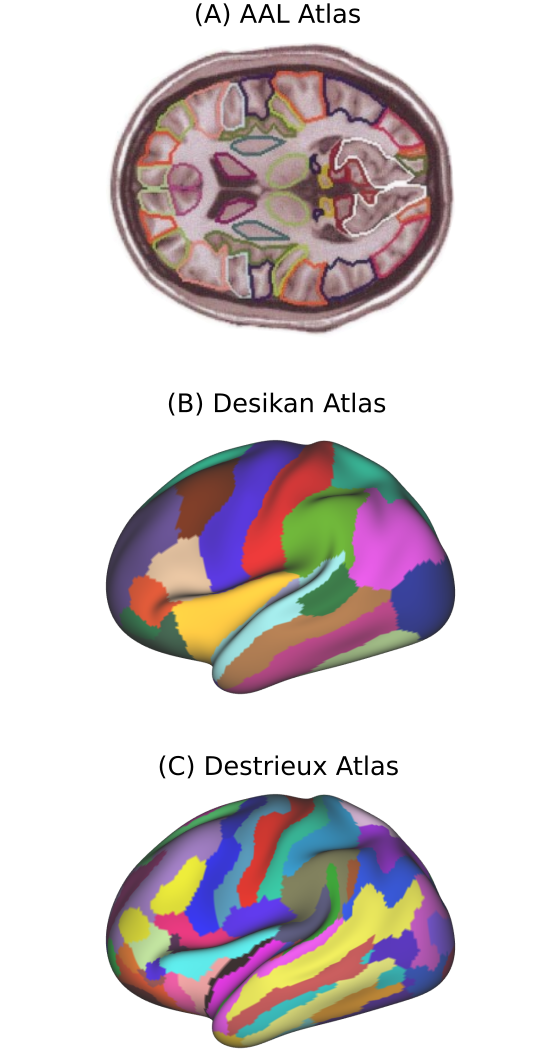
\includegraphics[width=0.49\textwidth]{4.brain_parcellation/img/anatomical.png}
    \caption{Examples of anatomical parcellations: (A) The AAL atlas~\cite{Landeau2002},
    (B) Desikan Atlas~\cite{Desikan2006}, and (C) Destrieux Atlas \cite{Destrieux2010}.
    The image of the AAL atlas was adapted from Landeau et al.~\cite{Landeau2002}.}
    \label{fig:brain_function}
\end{figure}

\begin{figure*}[t!]
    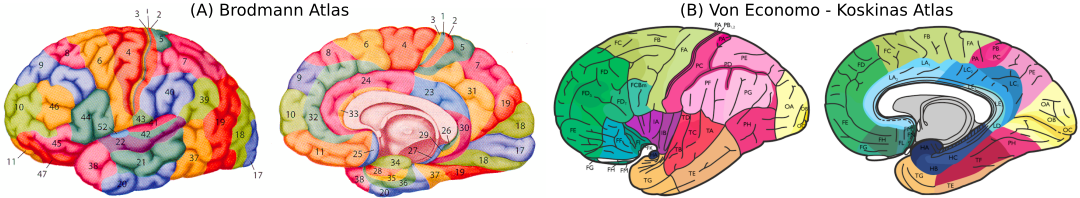
\includegraphics[width=\textwidth]{4.brain_parcellation/img/cytoarchitectonic.png}
    \caption{Two cytoarchitectonic parcellations: (A) The Brodmann atlas~\cite{Brodmann1909},
             and the von Economo and Koskinas atlas~\cite{VonEconomo1925}.}
    \label{fig:brain_function}
\end{figure*}


In recent years we have witnessed a rapid growth in the field of brain mapping,
driven by advances in Magnetic Resonance Imaging (MRI) and computational power.
In this chapter, we review the state-of-the-art in brain parcellation. We focus
on four different types: anatomical, functional, cytoarchitectonic and structural
parcellations. For each modality we explain the criteria behind them, and the
most notorious parcellations created based on them. We limit ourselves to present
parcellations without benchmarking them, for more information on benchmarking
please refer to the works of Thirion et al.~\cite{Thirion2014}, and Arslan et al.~\cite{Arslan2018}.
This review is by no means extensive, and more information can be found in
Amunts et al.\cite{Amunts2007}, Triarhou \cite{Triarhou2007} 
Jbabdi et al.~\cite{Jbabdi2013}, Arslan et al. \cite{Arslan2018},
de Reus et al.~\cite{DeReus2013}, and Eichhoff et al.~\cite{Eickhoff2015, Eickhoff2018a}.



\begin{figure*}[t]
    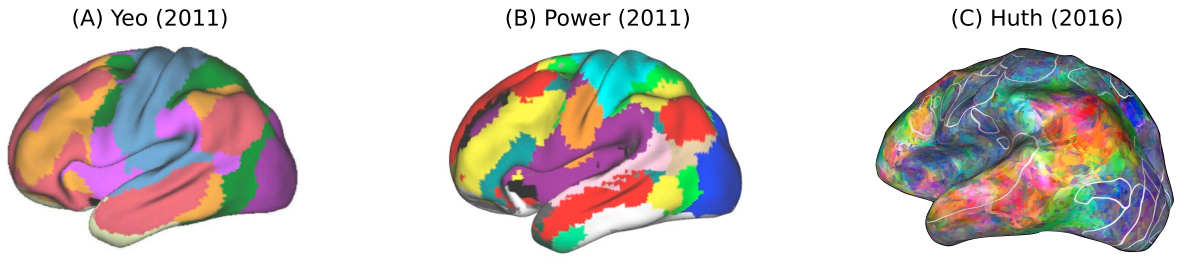
\includegraphics[width=\textwidth]{4.brain_parcellation/img/functional.png}
    \caption{Three functional parcellations of the brain: (A) A parcellation from
             the resting state fMRI of 1000 subjects by Yeo et al.~\cite{Yeo2011},
             (B) Functional networks defined by Power et al.~\cite{Power2011},
             and (C) a semantic map generated by Huth et al.~\cite{Huth2016}.}
    \label{fig:brain_function}
\end{figure*}

\section{Anatomical Parcellations}
\label{sec:anatomical}

In Anatomical parcellations, a region is characterized by its shape or
relative position in the brain. For example, in the Desikan atlas, the pars
opercularis region is defined as ``the first gyrus from the precentral
gyrus''~\cite{Desikan2006}. Anatomical parcellations were most probably the first
way to subdivide the brain, since references to anatomical landmarks can already
be found in ancient texts~\cite{Elsberg1945, Collice2008}.

Early anatomical atlases where solely based on the study of post-mortem brains,
being the most notable example being that of Talairach~\cite{Talairach1988}.
This atlas is based on the dissection of one human brain, and defines a
standardized coordinate system for neurosurgery. In moderns times, the
advent of MRI allowed to acquire massive amount
of brain images and create brain templates. A brain template is an image
which is a representative of the different brains on a population~\cite{Evans2012}. Two
examples of this are the Colin27 atlas~\cite{Collins1998}, based on the average
of 27 scans of a healthy subject, and the Montreal Neurological Institute (MNI) brain~\cite{Holmes1998},
which latest version (ICBM152) is based on the average of 152 healthy subjects images.
The parcellation of a brain template is, by definition, anatomically
consistent across subjects, and therefore is considered an atlas. This is the
case for example of the AAL atlas. The AAL atlas~\cite{Landeau2002}, is based on the manual
parcellation of the MNI brain atlas. The MNI single-subject main sulci were
first delineated and further used as landmarks for the 3D definition of 45
anatomical volumes of interest (AVOI) in each hemisphere.

When working only on the cortical surface, a well known anatomical atlas is that of
Desikan et al.~\cite{Desikan2006}. The Desikan et al. atlas is based on the segmentation
of a surface
template, generated from the average cortical folding of 40 healthy subjects
projected on a sphere. The template was manually segmented into 34 coarse 
structures per hemisphere. In order to label a new subject, the subject's cortical 
folding is projected into the sphere and aligned to the template, then 
the labels are mapped from the atlas to their cortical surface. The automatic
labeling method developed by Desikan et al. shows a great accuracy when labeling
new subjects~\cite{Desikan2006}. Another parcellation, made by 
Destrieux et al.~\cite{Destrieux2010}, presents a finer division of the cortex in
74 parcels per hemisphere. In the case of Destrieux et al., not only the cortical
folding is taken into account in order to label a region. Their
underlying probabilistic model takes into account information as: the curvature
and average convexity of the cortical surface, prior labeling probability for
that vertex, and as the labels of vertices in its local neighborhood.
Finally, the MarsAtlas~\cite{Auzias2016} by Auzias et al., uses the superior temporal
and inferior frontal sulcus as orthogonal axis to defines a grid over the cortex.
The rest of the sulci in the brain are aligned to this grid, and used to divide
the cortical surface in 41 regions. As shown in their paper, the resulting parcels
have good correspondence with some specific functional activations~\cite{Auzias2016}.

\section{Cytoarchitectonic Parcellations}
\label{sec:cytoarchitecture}

Cytoarchitectonic divisions of the brain are based solely in the cellular
composition of the cortex. In these atlases, a region is characterized by its
thickness and cellular organization. For example, Brodmann Area 4 has
``an unusually thick cortex; possess giant pyramidal cells,
and lacks both its internal and external granular layer''~\cite{Brodmann1909}.

Campbell~\cite{Campbell1905} is considered the first neuroanatomist to create
a cytoarchitectonic parcellation of the brain, composed of 14 regions with
different cellular composition. Shortly after Campbell, Elliot Smith\cite{Smith1907}
divided the cortex in 50 cytoarchitectonic areas. Two years after, Broadmann
published his cytoarchitectonic map of the brain~\cite{Brodmann1909}. Broadmann
defines 52 cortical regions, based
on the inspection trough microscope of cortical sections of post-mortem
brains of different species. In 1925 von Economo and Koskinas published
their Atlas of Cytoarchitectonics of the Adult Human Cerebral Cortex\cite{VonEconomo1925}.
Von Economo and Koskinas' atlas recognized 54 fundamental cytoarchitectonic areas with
76 variants and 107 modifications~\cite{Triarhou2007}. Their atlas is based on the
examination of mentally healthy subjects in the range of 30 to 40 years of age
through improved dissection and acquisition methodologies. The von Economo and 
Koskinas atlas is considered one of the most detailed and reproducible cytoarchitectonic
atlas available~\cite{Peden1947}.

More recently, Schleicher and Zilles~\cite{Schleicher1990} introduced a microstructural
metric, the gray level index, to create observer-independent parcellation methods.
Also, new cytoarchitectonic subdivisions of anatomical regions have been defined,
as the one by Eickhoff et al.~\cite{Eickhoff2008}, who studied neurotransmitter
receptors to map divisions in the visual cortex, or the atlas of the human
ventral visual stream obtained by Rosenke et al.~\cite{Rosenke2018} based on the
analysis of 11 post-mortem brains. Finally, new atlases have been created, such
as the  Jubrain~\cite{Mohlberg2012}, a cytoarchitectonic probabilistic map base of the
histological sections of ten post-mortem human brains; or the one by
Ding et al.~\cite{Ding2016}, based on the manual dissection and parcellation
of a 34 years old brain.

\section{Functional Parcellations}
\label{sec:functional}
Functional parcellations map cognitive functions to brain regions in the brain.
In this type of parcellation, each parcel is said to be specialized to serve one
cognitive function or to represent one essential aspect of the information
processed by it~\cite{Fuster2000}.

The first functional maps were derived from lesions. The language regions for
example, are named after Broca and Wernicke, who in the late 1800 reported
lesions in that region for aphasic patients~\cite{Johns}. Another example is
that of the human homunculus, a representation of motor and sensory functions,
which Penfied~\cite{Schleicher1990} mapped through experimenting with electrical
stimulation of different brain areas of patients undergoing open brain surgery.

The advent of functional MRI (fMRI) allowed to measure the blood-oxygen level
dependant signal. Knowing that the level of oxygen in blood increases when neurons activate,
fMRI can help to characterize which region of the brain active during specific
cognitive tasks, or during rest (resting state fMRI, rs-fmri). Many functional parceling
techniques rely on what is known as a functional connectivity matrix, a two
dimensional matrix that quantifies the correlation between the fMRI time series
of a set of brain regions. Such regions can be as big as pre-defined anatomical region
or as small as a single voxel. The simplest way to quantify connection between two regions is
by means of the Pearson's correlation between the fMRI time series at each region.

Most parceling techniques work by applying clustering algorithms to the
functional connectivity matrix. The most popular techniques use 
mixture models~\cite{Lashkari2010, Ryali2012}; ward clustering~\cite{Blumensath2013};
k-means clustering~\cite{Yeo2011, Shen2013, Kahnt2012}; hierarchical clustering~\cite{Eickhoff2011, Michel2011};
spectral clustering~\cite{Thirion2006, Craddock2011, Schaefer2017}, and
boundary detection~\cite{Gordon2016, Wig2014, Schaefer2017}.

Some widely used whole-brain atlases are those of Yeo et al.~\cite{Yeo2011},
Power et al.~\cite{Power2011}, Craddock~\cite{Craddock2011}. 
Yeo et al.~\cite{Yeo2011} propose to use k-means clustering on the average
rs-fmri connectivity from 1000 subjects. The results yield two parcellations,
with 7 parcels and 17 parcels respectively, that show to be reproducible across
groups of subjects. Power et al.\cite{Power2011} use graph analysis and subgraph
detection techniques in order to characterize functional subnetworks in the
connectivity graph. Finally, Craddock et al.~\cite{Craddock2011}
use spectral clustering on rs-fmri connectivity to create fine-grained parcellations
ranging form 200 to 1000 parcellations.

Other papers worth mentioning are those of Deen et al.~\cite{Deen2011} and Hurt
et al.~\cite{Huth2016}. Deen et al. present a functional division
of the insula, that has been proved to be highly reproducible across subjects
and studies. Meanwhile, Huth et al. present an innovative atlas which maps semantic
domains (e.g. violent, temporal, professional) across the cortex~\cite{Huth2016}.
They use voxel-wise modelling of functional MRI (fMRI) data collected while 
subjects listened to hours of narrative stories.

\begin{figure*}[t]
    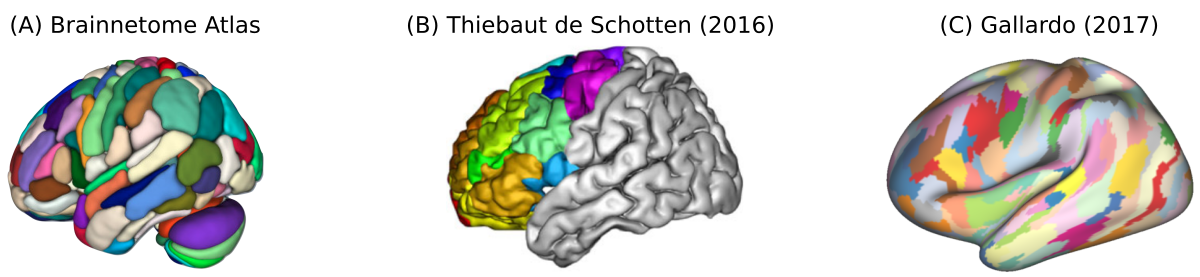
\includegraphics[width=\textwidth]{4.brain_parcellation/img/structural.png}
    \caption{Examples of structural parcellations of the brain: (A) The Brainnetome
             Atlas by Fan et al.\cite{Fan2016}, (B) A parcellation of the
             frontal lobe by Thiebaut de Schotten et al.~\cite{ThiebautdeSchotten2016} and (C)
             a groupwise parcellation from Gallardo et al.~\cite{Gallardo2017a}.}
    \label{fig:brain_function}
\end{figure*}

\section{Structural Parcellations}
\label{sec:structural}
Structural parcellations are based on estimations of axonal connectivity. On
a structural parcellations, each parcels presents a distinct pattern of
connectivity with respect to a predefined set of regions of interest. For example,
area MFG-5 of the Brainnetome atlas has ``connections 
with the major frontal subregions, the limbic area, the parietal subregions
and the subcortical connections with the thalamus and basal ganglia subregions''\cite{Fan2016}.

The first structural atlases were defined on macaque by means of chemical tracing~\cite{Stephan2013}.
Advances in Diffusion MRI (dMRI) and tractography algorithms enabled the in vivo
exploration of axonal connectivity on the human brain. This allowed to non-invasively
estimate connectivity between different brain regions. As with functional data,
the most common way to generate a parcellation is by first computing a connectivity matrix
between regions (in this case, a structural connectivity matrix), and then parcellate it using
some clustering technique.

The most popular techniques to parcellate the structural connectivity matrix
are thresholding~\cite{Behrens2003}; mixture models~\cite{Jbabdi2009, Clarkson2010, Paristot2015};
k-means~\cite{Anwander2006}; Principal Component Analysis~\cite{ThiebautdeSchotten2014, ThiebautdeSchotten2016};
Independent Component Analysis\cite{Muircheartaigh2018}; spectral reordering\cite{Bajada2017}; spectral clustering\cite{Fan2016};
watershed based dimension reduction\cite{Roca2009, Lefranc2016}; and hierarchical clustering\cite{Moreno-Dominguez2014, Gallardo2017a}.

Notables work are those of Behrens et al.\cite{Behrens2003}, Anwander et al.~\cite{Anwander2006},
Thiebaut et al.~\cite{ThiebautdeSchotten2016}, Moreno-Dominguez et al.~\cite{Moreno-Dominguez2014},
Bajada et al~\cite{Bajada2017} and Fan et al.~\cite{Fan2016}.
Behrens et al.~\cite{Behrens2003} define a structural parcellation of the thalamus.
Using tractography, they compute how a set of seed voxels in the thalamus are
connected to anatomically defined cortical regions. Then, they assign to each
seed-voxels the label of the cortical region with which it connects the most.
Anwander et al.~\cite{Anwander2006}
uses k-means clustering over the connectivity matrix of Broca's area, obtaining
a division in 3 regions, consistent with cytoarchitectonic divisions.
Thiebaut de Schotten et al.~\cite{ThiebautdeSchotten2016}
parcellate the frontal lobe in 12 regions by means of principal component analysis,
and shows its reproducibility across subjects and datasets.
Moreno-Dominguez creates a hierarchical parcellation of the brain by using
ward clustering~\cite{Moreno-Dominguez2014}, allowing to obtain a parcellation
of the brain with different granularities. Fan et al.\cite{Fan2016} use
spectral clustering over connectivity data to subdivide regions of the Desikan
atlas~\cite{Desikan2006}, obtaining a parcellation with 210 cortical areas and
36 subcortical regions. Finally, Bajada et al.~\cite{Bajada2017} take a different
approach and use spectral reordering to create a soft parcellation over the
temporal lobe. This allows to have parcels that diffuse into each other, instead
of sharp boundaries dividing them.

\begin{figure*}[t]
    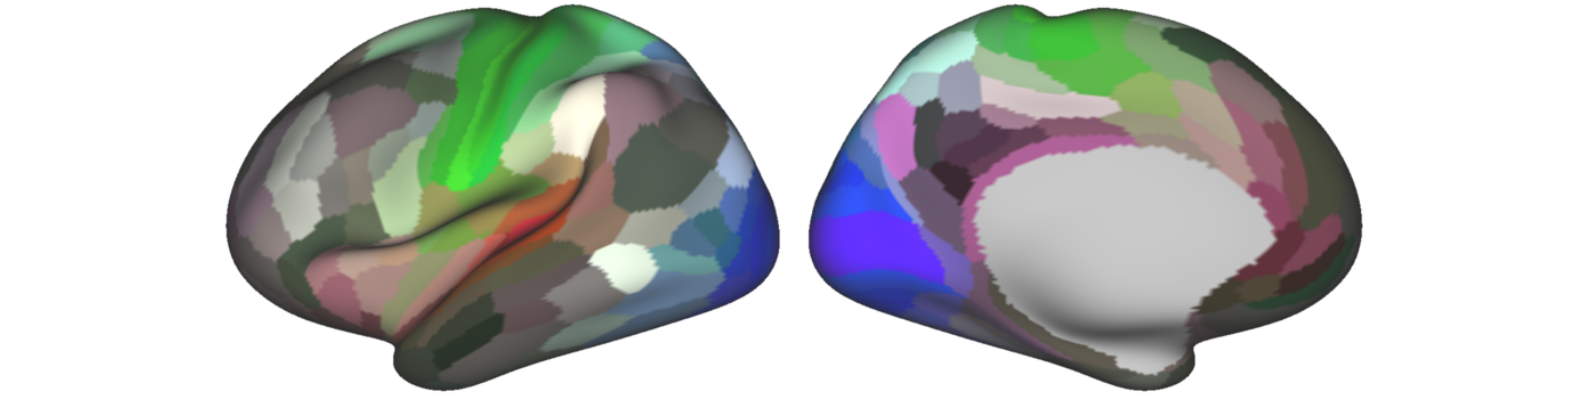
\includegraphics[width=\textwidth]{4.brain_parcellation/img/multimodal.png}
    \caption{The atlas of Glasser et al.~\cite{Glasser2016} is a well-known
             multi-modal parcellation of the brain.}
    \label{fig:brain_function}
\end{figure*}

\section{Multi-modal}
\label{sec:multimodal}
Multi-modal parcellations are relatively new in the field of brain mapping.
By combining information from different neuroimaging methodologies, multi-modal
techniques create regions which boundaries are consistent with multiple
independent neurobiological properties.

Examples of multi-modal parcellations are those of Diez et al. \cite{Diez2014},
Parisot et al. \cite{Parisot2017}, and the Glasser-van Essen atlas.~\cite{Glasser2016}. 
Diez et al. \cite{Diez2014} merges structural connectivity and functional
connectivity in order to compute common structure-function modules (SFMs).
Their methodology defines a cross-modularity index, that indicates how
modular a parcellation is with respect to both matrices, and how similar is the
internal connectivity in both modalities. By searching for the parcellation
that maximizes this index, they obtain a cortical parcellation with 20 structure-function
modules. Parisot et al. \cite{Parisot2017} starts by computing a set of
parcellations from fMRI, rs-fMRI, estimations of myelin maps, and tractography.
These parcellations are then fused based on their local reliabilities by means of
mixture models. The fused parcellation is iteratively refined, forcing 
the parcellations to converge towards a set of mutually informed modality specific
parcellations. Finally, Glasser et al.~\cite{Glasser2016}
divide the cortex in 180 regions which borders are consistent with: 
myelin content maps, cortical thickness maps, and task-fMRI activations. Their
approach combines a semi-automated prior segmentation with a machine learning
algorithm to optimize the border placement.

\vspace{10px}

\section{Discussion}

The brain is a highly complex cellular network, in order to study it, some
way of dimensionality reduction is needed. Given that neurons tend to organize
and activate in a spatially coherent way, it is possible to model the brain as a
mosaic of regions. As seen in sections \ref{sec:anatomical}-\ref{sec:multimodal},
the brain is divided on criteria such as anatomy, function, cytoarchitecture or
extrinsic connectivity. Each criterion sees the brain in a different way, and
relies on different acquisition methods. 

Cytoarchitectonic parcellations denote the cellular composition of the brain,
therefore, they are the perfect candidate to abstract populations of neurons.
Also, the close relationship between cytoarchitecture and brain function\cite{Amunts2007}
makes them useful as functional parcellations.
However, when using these parcellations is important to acknowledge their limitations.
First, existent cytoarchitectonic maps do not cover the whole brain, in fact, only 
approximately 40\% of the cortical surface has been mapped~\cite{Amunts2007}. Second, all cytoarchitectonic atlases are based on just
a few post-mortem brains, making them hard to represent a population. This is
product of the complex process of dissecting a brain, delimiting its regions,
and registering the results to a common space. The whole process requires in most
cases one person year of work per region. Finally, and most importantly, given the
amount of variability~\cite{Zilles2013} in different subjects, registering a 
cytoarchitectonic atlas to a new brain based on anatomical features does not
guarantee the correct localization of the areas. Until now, post-mortem dissection
remains as the only way to correctly locate cytoarchitectonic areas.

Anatomical parcellations are based on fairly common brain landmarks, making them
highly reproducible across subjects, but incurring in the trade-off of having coarse
brain regions. Nowadays, the general function of most anatomical parcels is
known, making them useful to use as a gross first delimitation of the brain
when studying particular brain functions. When using anatomical atlases, it is
important to remind that only the borders of a few architectonically
defined areas show a sufficiently precise association with sulci~\cite{Amunts2007}.
Hence, anatomical atlases are not good candidates to abstract populations
of neurons in the brain.

Functional parcellations map cognitive functions to brain locations, and are
a key element to understand how the brain works. Many functions have been shown
to be consistent across subjects~\cite{Johns, Penfield1954, Yeo2011},
and the close relationship with cytoarchitecture makes them good candidate to
abstract population of neurons. However, functional parcellations are based
on the modular paradigm, which states that one brain region is specialized
on one cognitive function. New evidence suggests that the modular paradigm has serious
limitations and might in fact be misleading~\cite{Bressler2010}.

Structural parcellations define regions with homogeneous axonal connectivity.
Axonal connectivity plays a fundamental role in the interaction between brain
regions~\citep{Schmahmann2006}. Moreover, long-range axonal connections are
strongly related to brain function~\citep{Passingham2002}, and
cytoarchitecture~\cite{Muircheartaigh2018}. The downside is that tractography,
the underlying technique to estimate axonal connectivity, is still 
not mature enough. In fact, recent studies show that state-of-the-art
tractography algorithms create four times more false positives than true
positives~\cite{Hein2016}.

Multi-modal parcellations combine information from different neuroimaging methodologies,
in order to create regions consistent with multiple neurobiological properties.
Their main limitation is that sometimes, regions tend to over represent one
modality. A clear example is the subdivision of the precentral and poscentral
gyrus in the atlas of Glasser et al.~\cite{Glasser2016}. Even when motor tasks
are used during the construction of the atlas, the resulting subdivisions of
both motor and sensory cortex appear to be driven by myelination. This
result is inconsistent with the well known functional subdivision of both motor
and sensory cortex.

We finish this review by highlighting that, if a universal parcellation of
the brain exists, it has not been found yet. Meanwhile, different atlases and
techniques to divide the brain coexist. As discussed above, parcellations based
on different criteria have different advantages and disadvantages. At the end,
which parcellation to use in practice will heavily depend on the hypothesis
and the goal of the study to be done.

\section{Conclusion}
In this chapter we presented parcellations based on different criteria and
discussed their advantages. In the following chapter we will introduce the
first contribution of this thesis: a parsimonious model for the long-range
connectivity and a whole-brain structural parceling technique. We will show
that our technique creates parcels in agreement with anatomical, structural
and functional parcellations existent in the literature.

\chapterbib
